\subsection{Reaction decomposition of the $d(K^-, n \pi^+ \pi^-)"n"$}
\begin{figure}[htbp]
  \begin{tabular}{ccc}
    \begin{minipage}{0.33\hsize}
      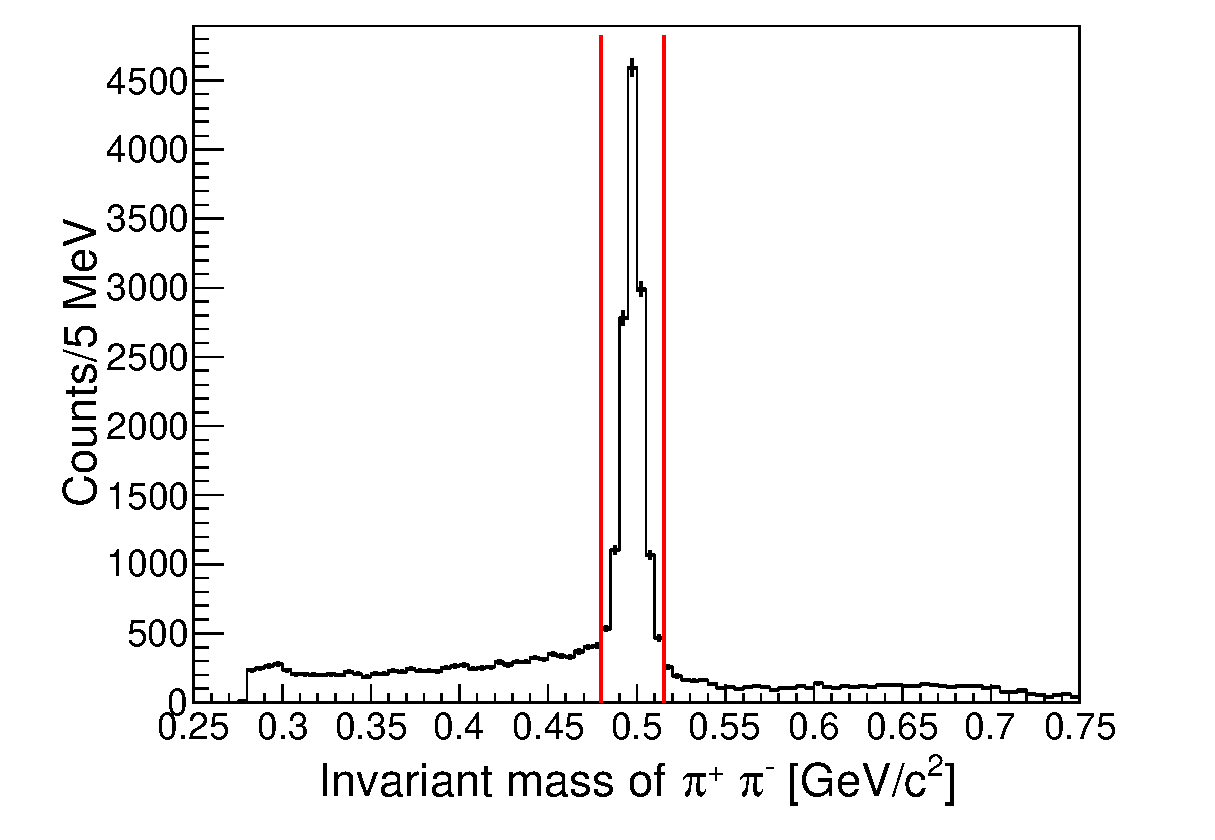
\includegraphics[width=4cm]{../pic/Run78/KN_ana_NC170_2sigma/IM_pipi_woFit.eps}
    \end{minipage}
    \begin{minipage}{0.33\hsize}
      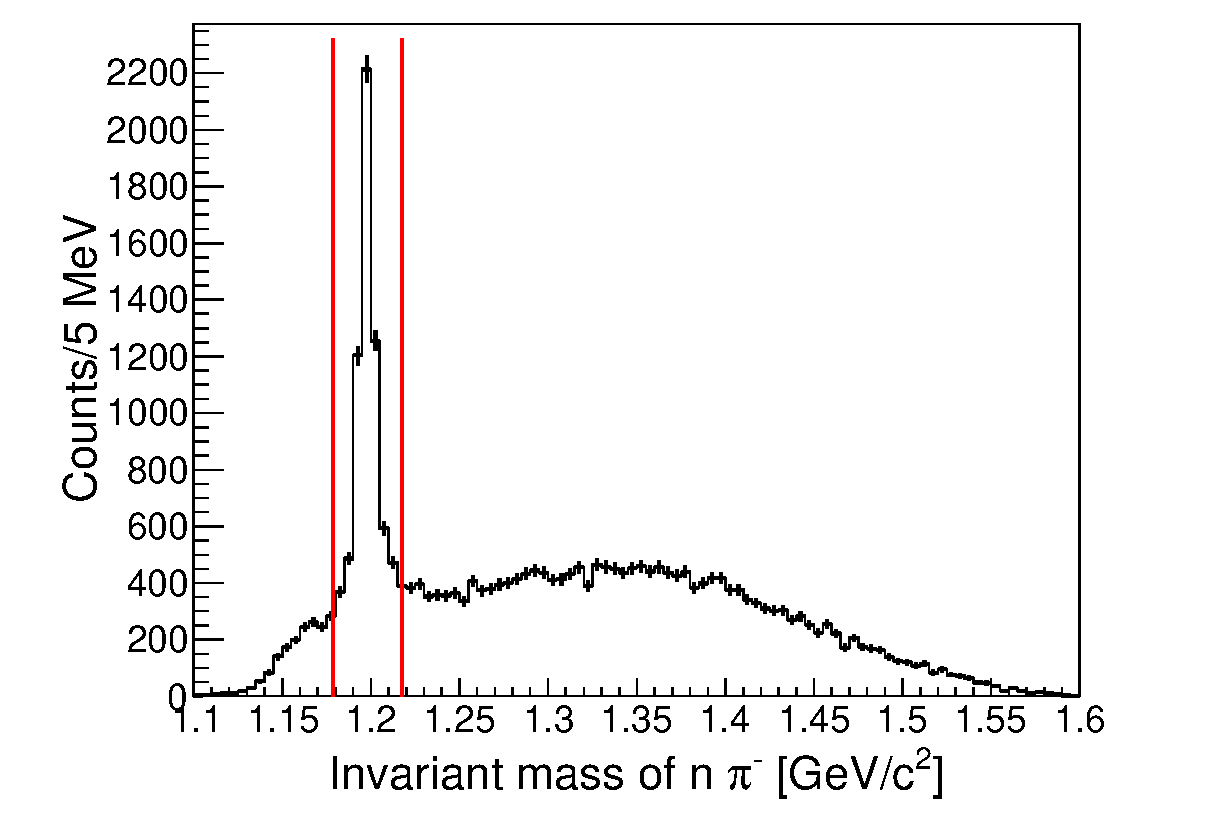
\includegraphics[width=4cm]{../pic/Run78/KN_ana_NC170_2sigma/IM_npim_woFit.eps}
    \end{minipage}
    \begin{minipage}{0.33\hsize}
      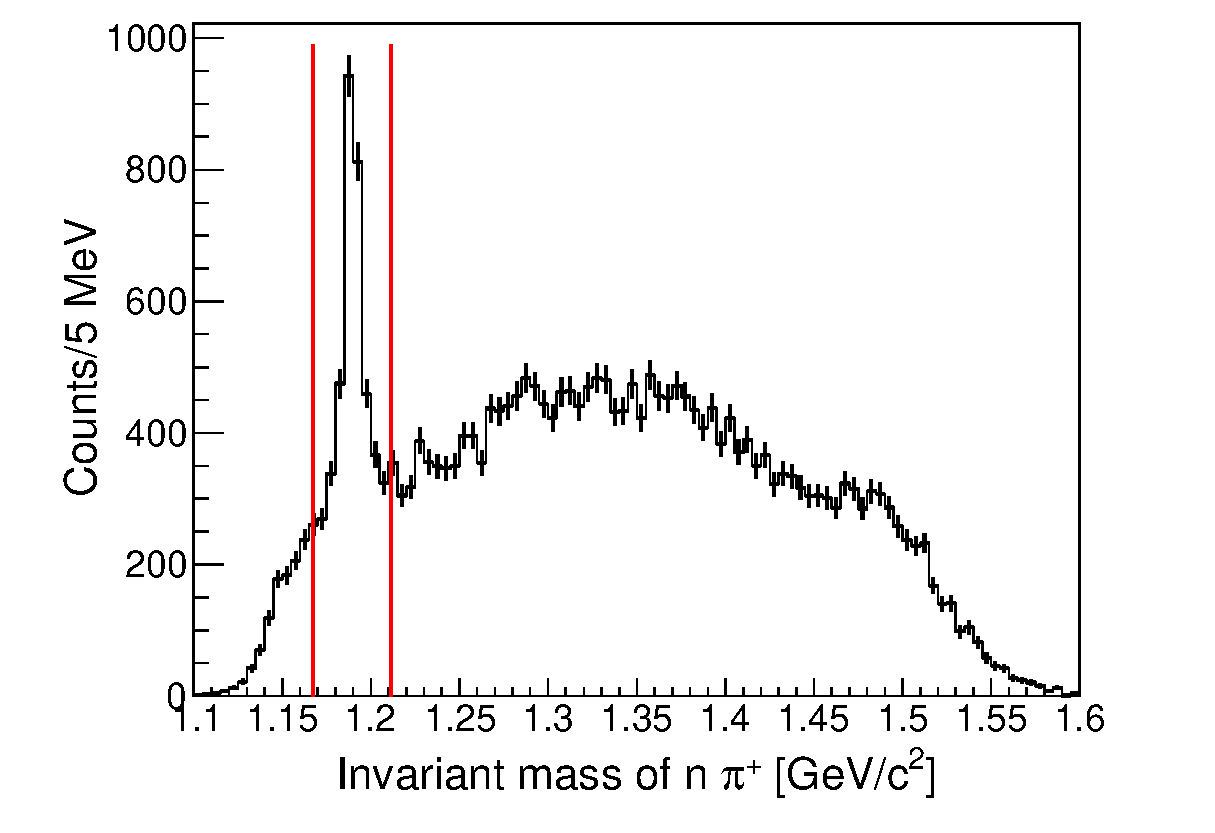
\includegraphics[width=4cm]{../pic/Run78/KN_ana_NC170_2sigma/IM_npip_woFit.eps}
    \end{minipage}
  \end{tabular}

  \caption{
    These figures show invariant masses of $\pi^+ \pi^-$, $n \pi^-$ and $n \pi^+$ in $K^- d \rightarrow n \pi^+ \pi^- n$ final state identified events, respectively.
    Red lines indicate select region for $K^0$, $\Sigma^-_{forward}$ and $\Sigma^+_{backward}$, respectively.
  }
  \label{fig:KNpipi_IM}
\end{figure}

\begin{figure}[htbp]
  \centering
  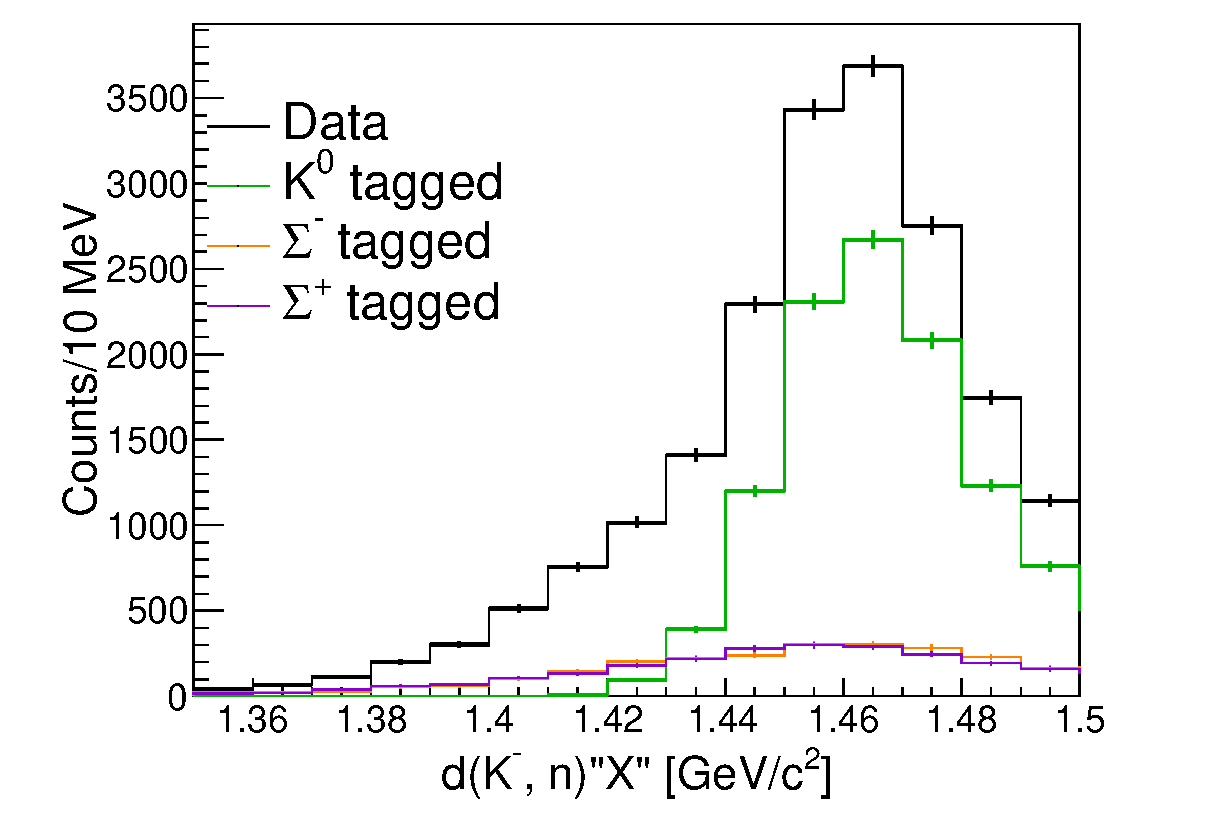
\includegraphics[width=12cm]{../pic/Run78/KN_ana_NC170_2sigma/KN_MM_all.eps}
  \caption{
    This figure shows the missing mass of $d(K^-, n)$ identified $d(K^-, n \pi^+ \pi^-)"n"$ final state.
    Color plots show $K^-$ and $\Sigma_{forward}$ identifed by invariant mass of detected particles.
    $K^0$ contamination is remained in quasi-elastic region.
    $\Sigma_{forward}$ contaminations are negligebly small.
  }
  \label{fig:KN_MM_npipin}
\end{figure}

In the $d(K^-, n \pi^+ \pi^-)"n"$ final state, following 5 reactions was expected.
\begin{eqnarray}
  K^- d \rightarrow K^0 n n \label{eq:KD_K0nn}\\
  K^- d \rightarrow \Sigma^+_{froward} \pi^- n \label{eq:KD_pimSpf} \\
  K^- d \rightarrow \Sigma^-_{froward} \pi^+ n \label{eq:KD_pipSmf} \\
  K^- d \rightarrow \Sigma^+ \pi^- n_{forward} \label{eq:KD_pimSp} \\
  K^- d \rightarrow \Sigma^- \pi^+ n_{forward} \label{eq:KD_pipSm}
\end{eqnarray}
In reaction.(\ref{eq:KD_pimSpf})-(\ref{eq:KD_pipSmf}), the $\Sigma^{\pm}_{forward}$ means the detected neutron by the NC decayed from $\Sigma_{\pm}$.
These reaction were identified from invariant masses of $n$ and $\pi^{\pm}$ as shown in the center and right figure of Fig\ref{fig:KNpipi_IM}.
In the reaction.(\ref{eq:KD_K0nn}), the $K^0$ was identified from the invariant mass of $\pi^+$ and $\pi^-$ as shown in the left figure of Fig\ref{fig:KNpipi_IM}.
In reaction.(\ref{eq:KD_pimSp})-(\ref{eq:KD_pipSm}) which were so-called the $d(K^-, n)"\pi^{\mp}\Sigma^{\pm}"$ modes,
the injected $K^-$ was recoild, took the strangness, and scattered with the residual nucleon to become the $\pi\Sigma$.
So, these reactions were the 2-step reaction and the signal in this thesis.

Fig\ref{fig:KN_MM} shows the missing mass of the $d(K^-, n)$ identified the $d(K^-, n \pi^+ \pi^-)"n"$.
The spectra tagged reconstructed hyperons were indicated in the same figure.
The $d(K^-, n)"\pi^{\mp}\Sigma^{\pm}"$ mode were events rejected the $K^0$ and the $\Sigma^{\pm}_{forward}$, which was plotted in Fig\ref{fig:KN_MM_woAll}.
In the same figure, the	contamination from the other 3 reactions was also plotted which was estimated by the template fitting to decompose each reaction, which was explained after.

\begin{figure}[htbp]
  \centering
  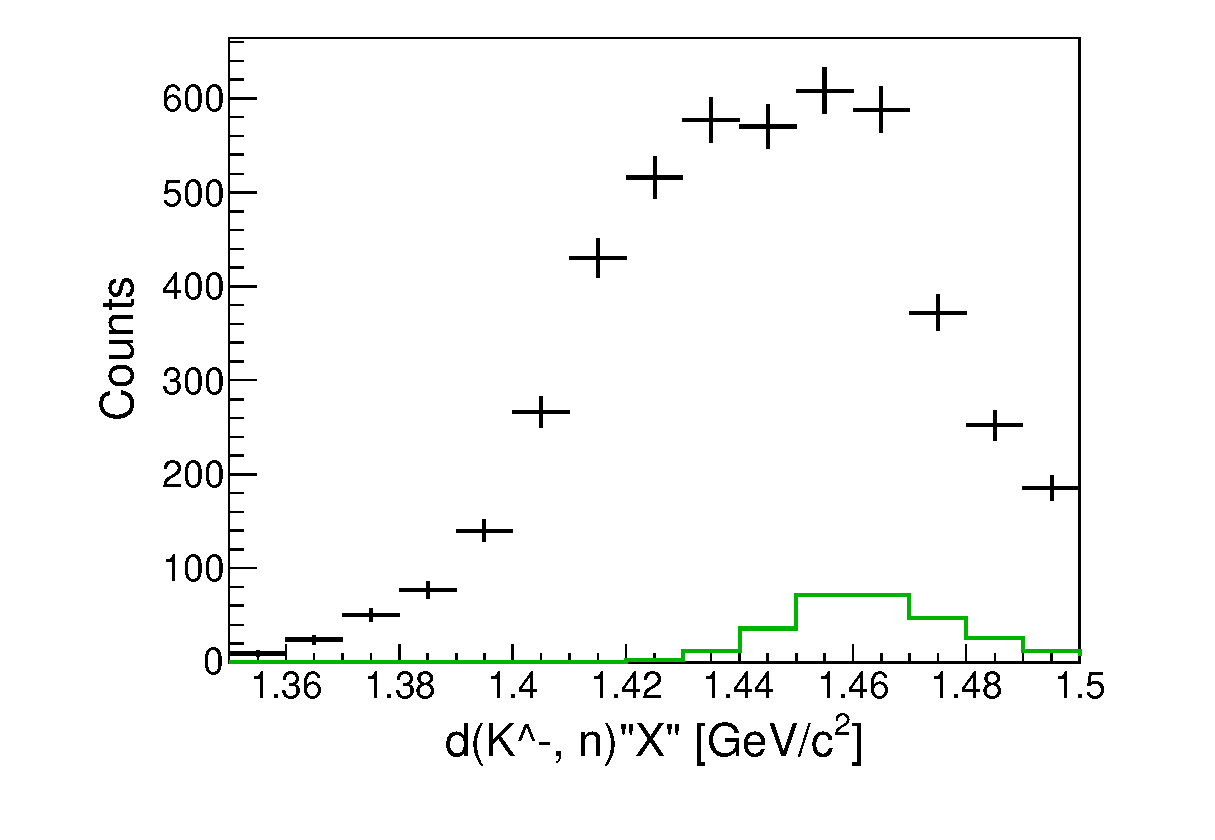
\includegraphics[width=12cm]{../pic/Run78/KN_ana_NC170_2sigma/KN_MM_woAll.eps}
  \caption{
    The figure shows $d(K^-, n)"\pi^{\pm}\Sigma^{\mp}"$ which was identified to reject events identified $K^0$ and $\Sigma_{forward}$ from detected particles.
    Color plots indicate contamination estimated by the template fitting of invariant masses.
  }
  \label{fig:KN_MM_woAll}
\end{figure}

\begin{figure}[htbp]
  \begin{tabular}{ccc}
    \begin{minipage}{0.33\hsize}
      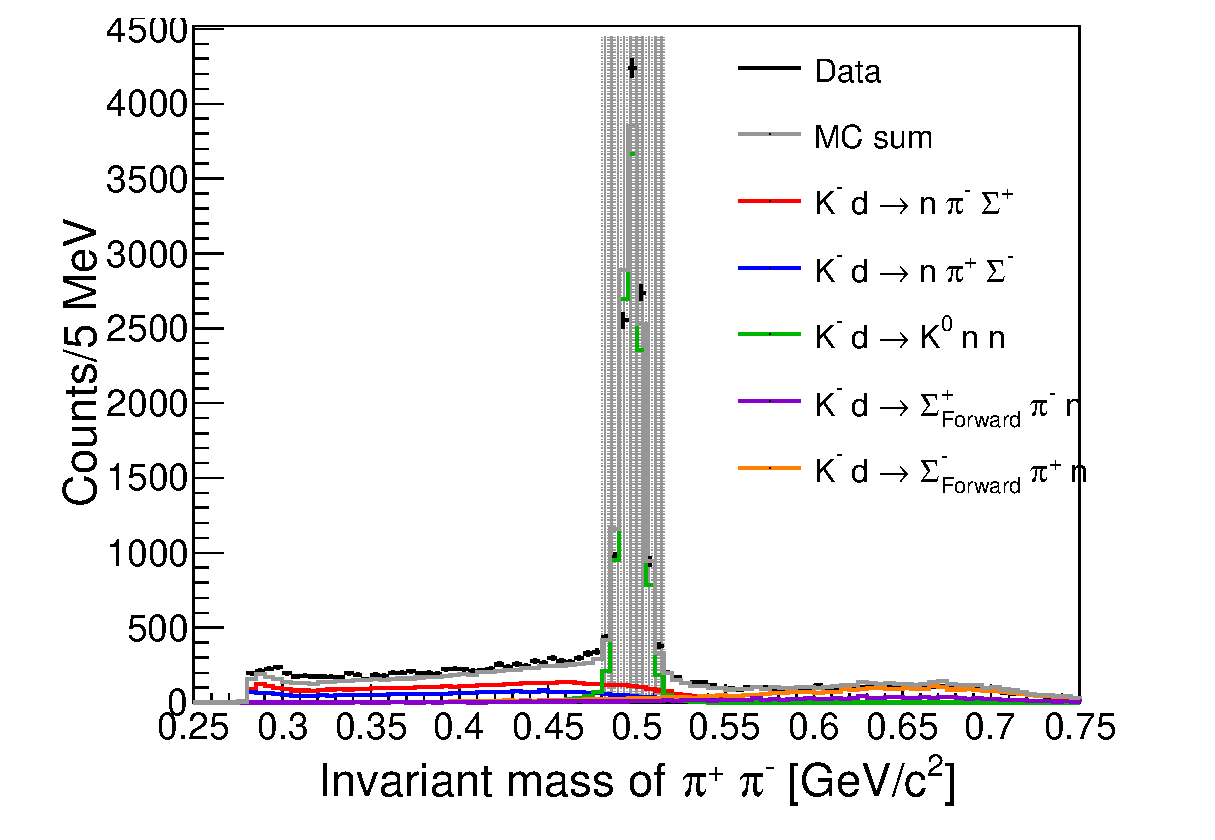
\includegraphics[width=4cm]{../pic/Run78/KN_ana_NC170_2sigma/IM_pipi.eps}
    \end{minipage}
    \begin{minipage}{0.33\hsize}
      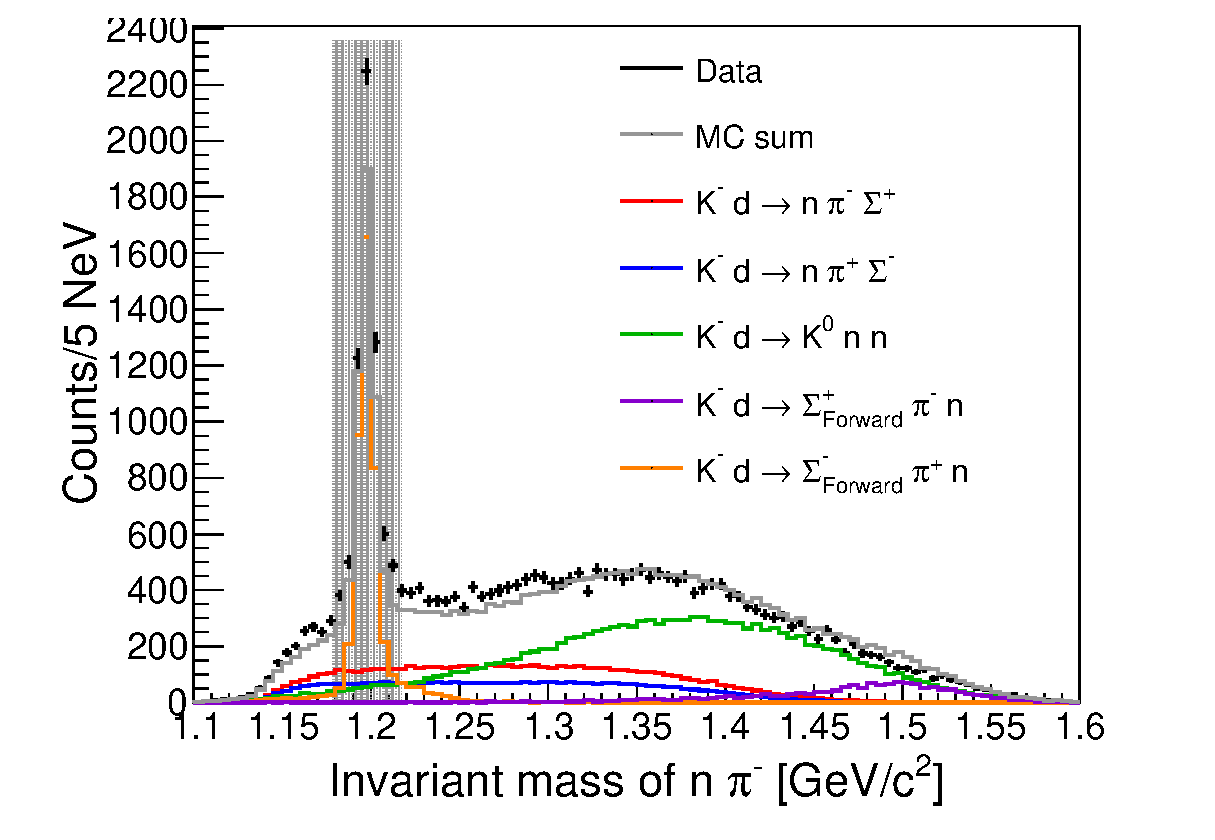
\includegraphics[width=4cm]{../pic/Run78/KN_ana_NC170_2sigma/IM_npim.eps}
    \end{minipage}
    \begin{minipage}{0.33\hsize}
      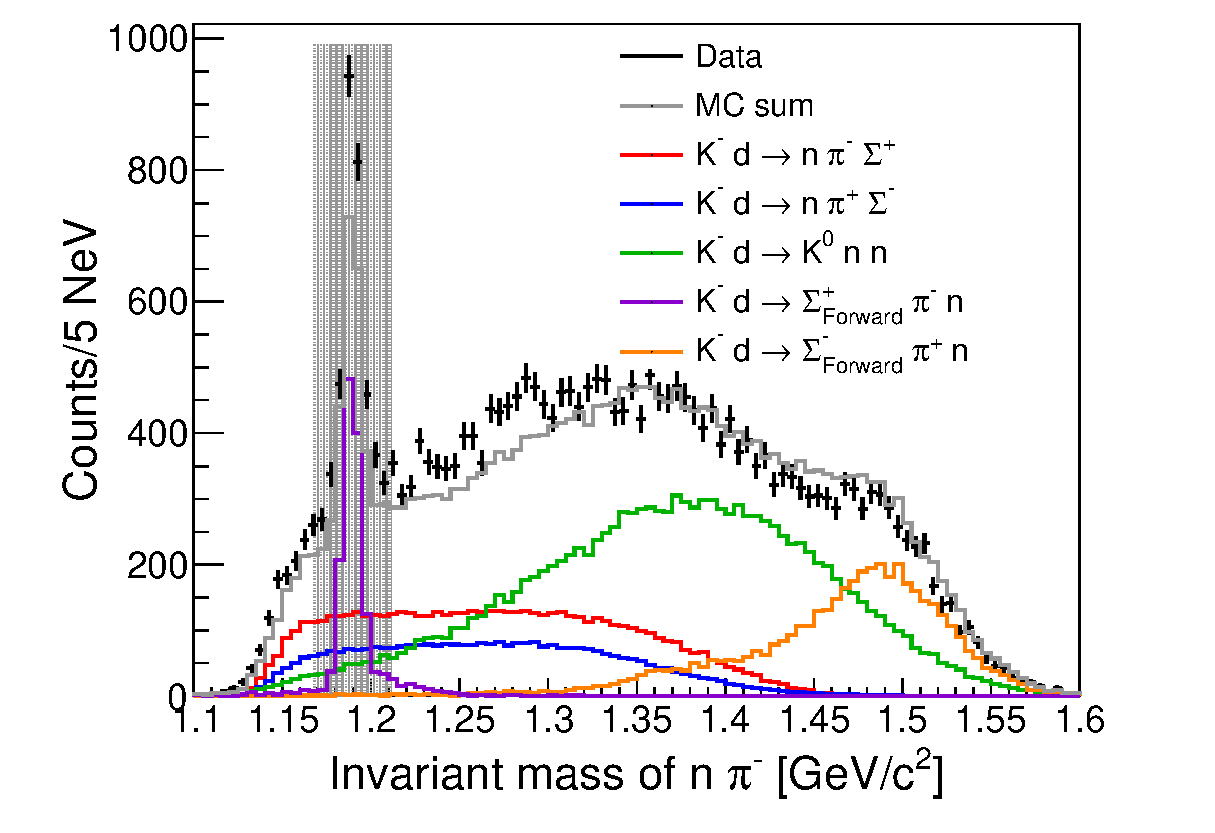
\includegraphics[width=4cm]{../pic/Run78/KN_ana_NC170_2sigma/IM_npip.eps}
    \end{minipage}
  \end{tabular}
  \caption{
    These figures shows invariant masses of $\pi^+ \pi^-$, $n \pi^-$ and $n \pi^+$ with fitting result of 5 reactions.
  }
  \label{fig:IM_fit}
\end{figure}

\begin{figure}[htbp]
  \begin{tabular}{cc}
    \begin{minipage}{0.5\hsize}
      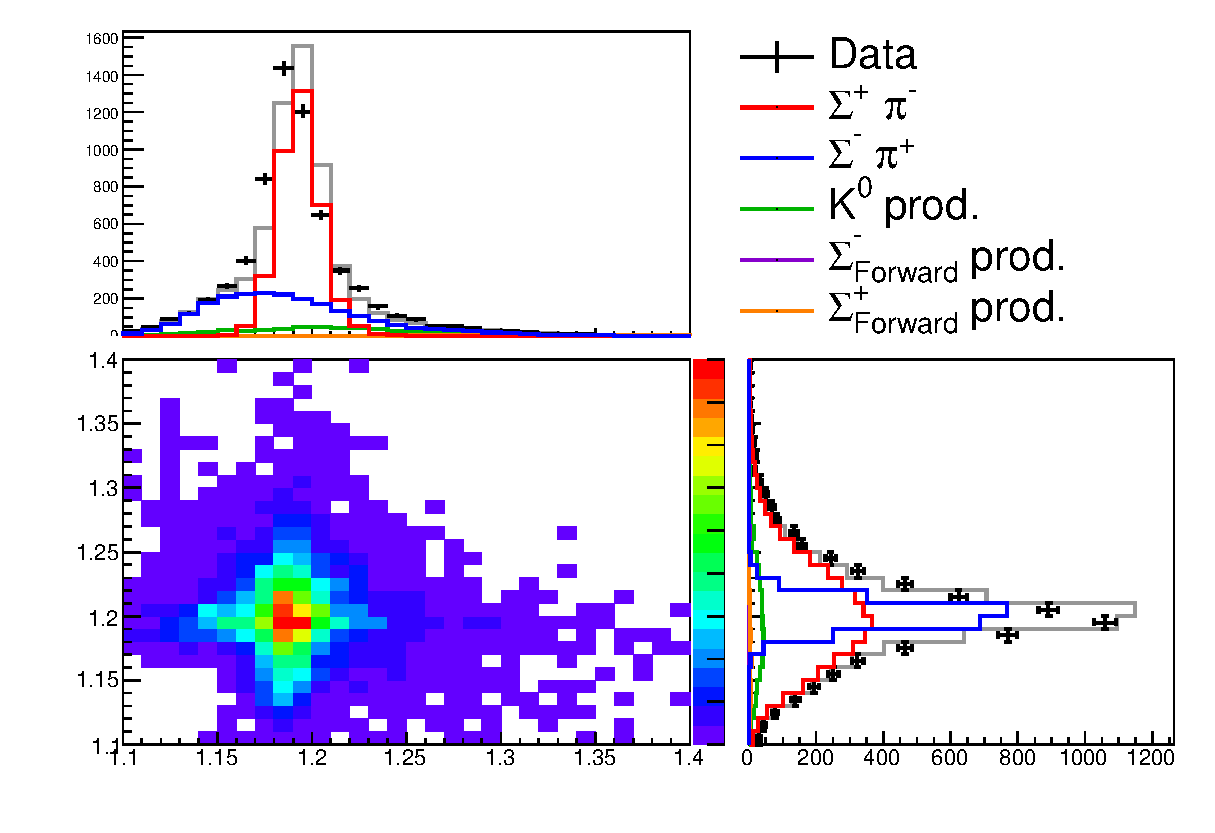
\includegraphics[width=6.5cm]{../pic/Run78/KN_ana_NC170_2sigma/KNpim_KNpip_MM.eps}
    \end{minipage}
    \begin{minipage}{0.5\hsize}
      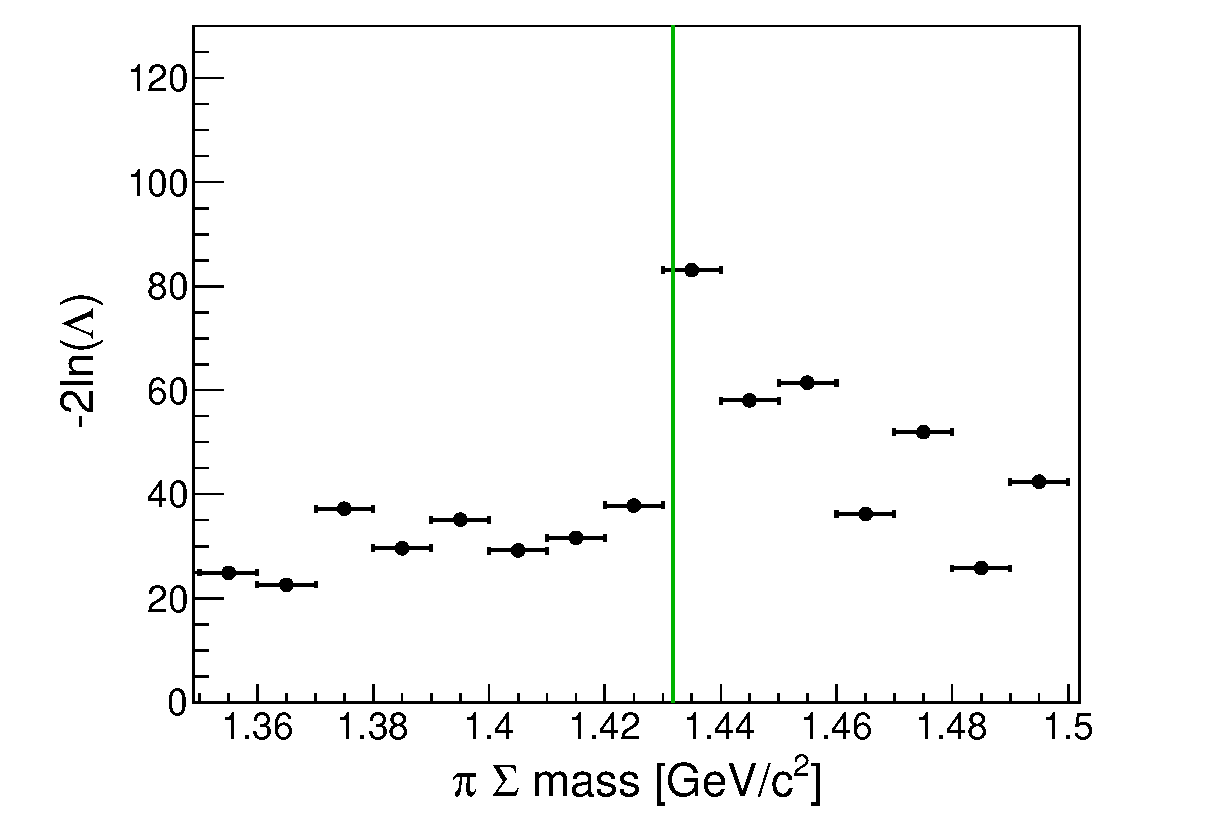
\includegraphics[width=5.5cm]{../pic/Run78/KN_ana_NC170_2sigma/Chi2.eps}
    \end{minipage}
  \end{tabular}
  \caption{
    This figure indicates summed up fitting result and log-likelihood value of each bins.
  }
  \label{fig:KNpi_MM_fit}
\end{figure}

\begin{figure}[htbp]
  \begin{tabular}{ccc}
    \begin{minipage}{0.33\hsize}
      \includegraphics[width=4cm]{../pic/Run78/KN_ana_NC170_2sigma/KNpi_MM_0.eps}
    \end{minipage}
    \begin{minipage}{0.33\hsize}
      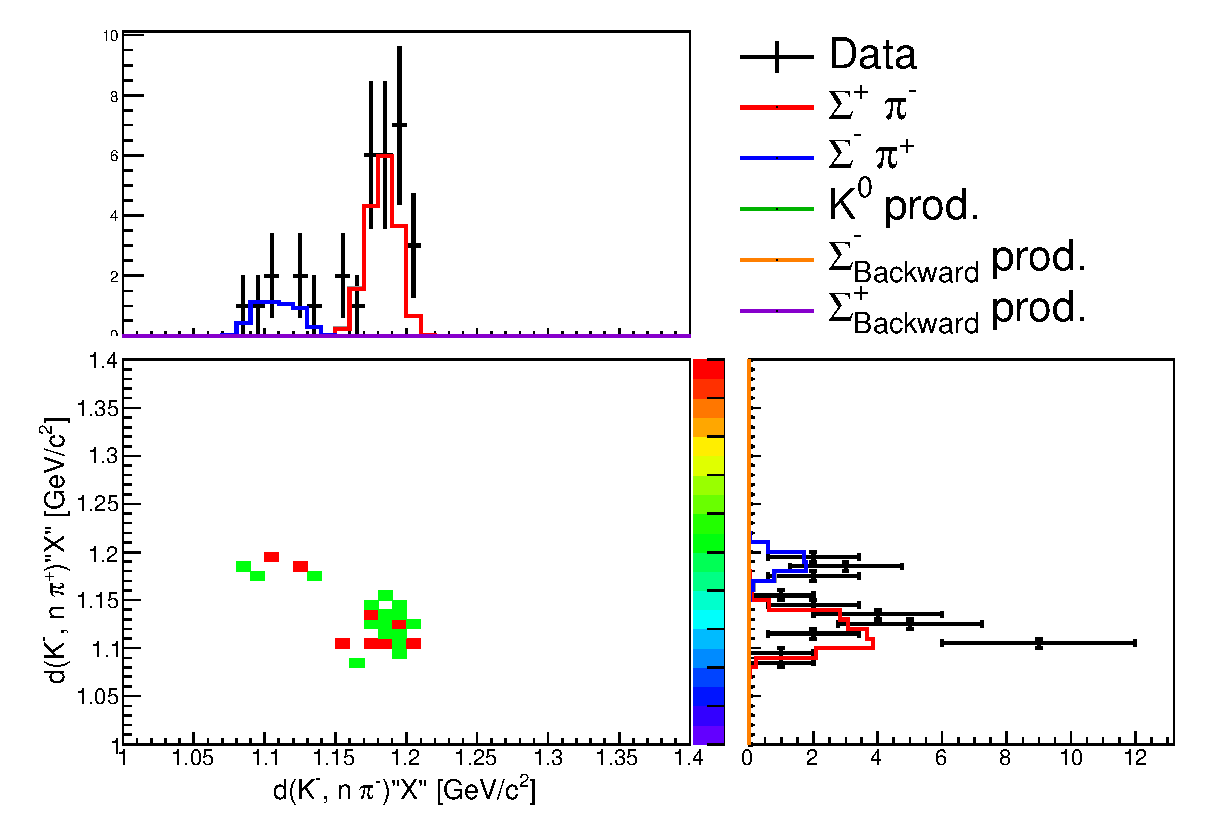
\includegraphics[width=4cm]{../pic/Run78/KN_ana_NC170_2sigma/KNpi_MM_1.eps}
    \end{minipage}
    \begin{minipage}{0.33\hsize}
      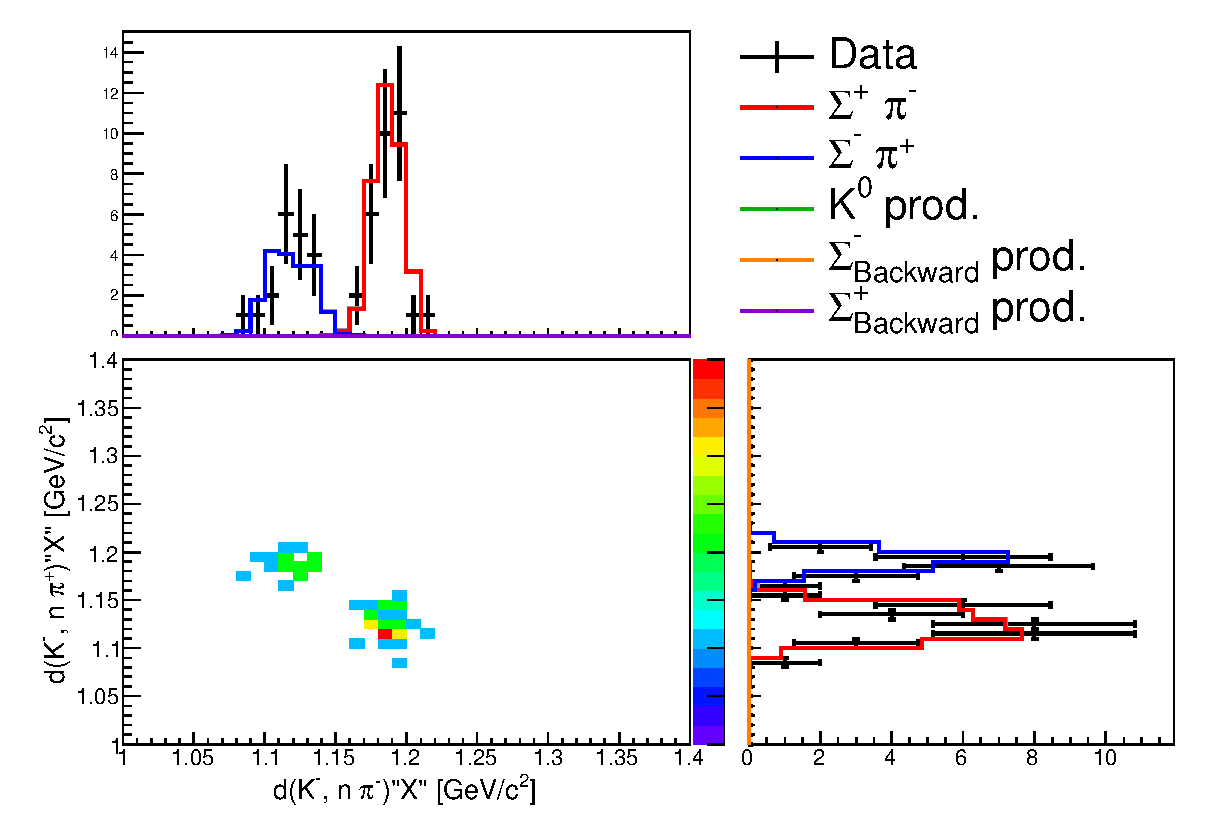
\includegraphics[width=4cm]{../pic/Run78/KN_ana_NC170_2sigma/KNpi_MM_2.eps}
    \end{minipage}
  \end{tabular}

  \begin{tabular}{ccc}
    \begin{minipage}{0.33\hsize}
      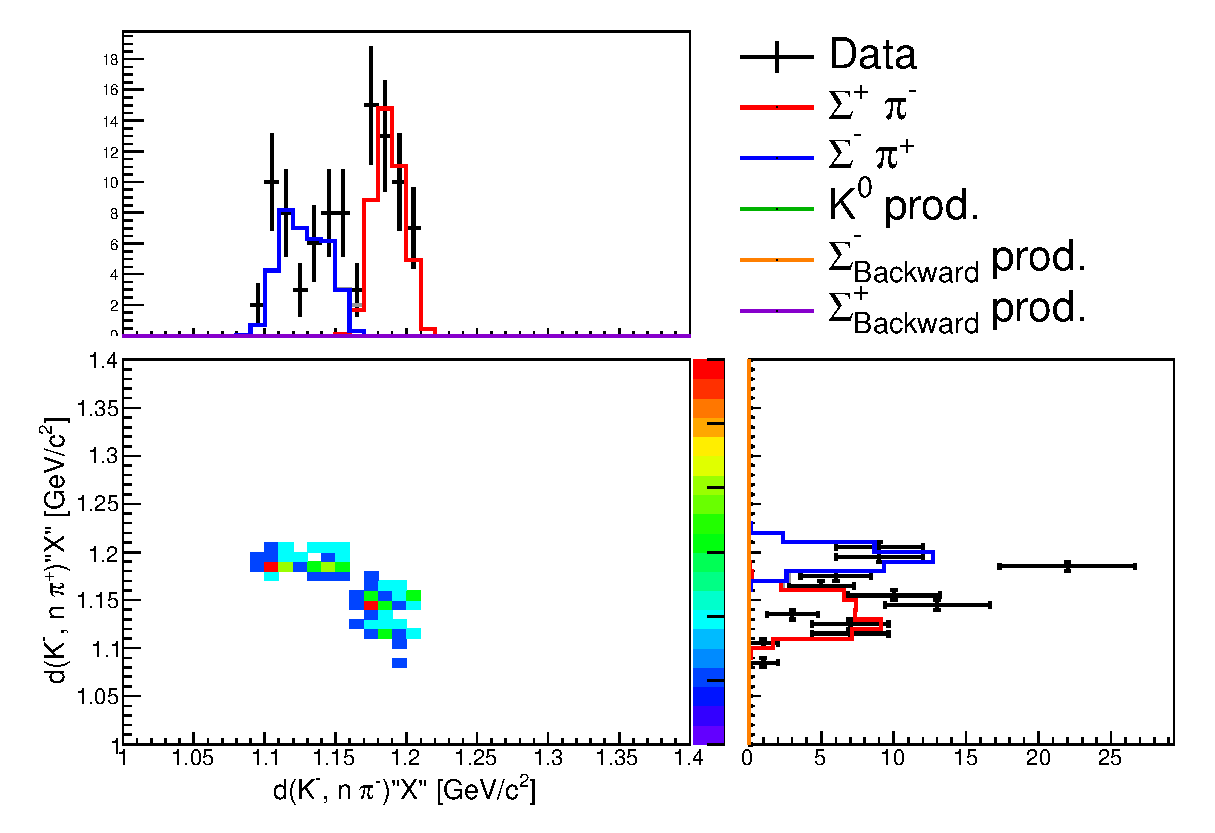
\includegraphics[width=4cm]{../pic/Run78/KN_ana_NC170_2sigma/KNpi_MM_3.eps}
    \end{minipage}
    \begin{minipage}{0.33\hsize}
      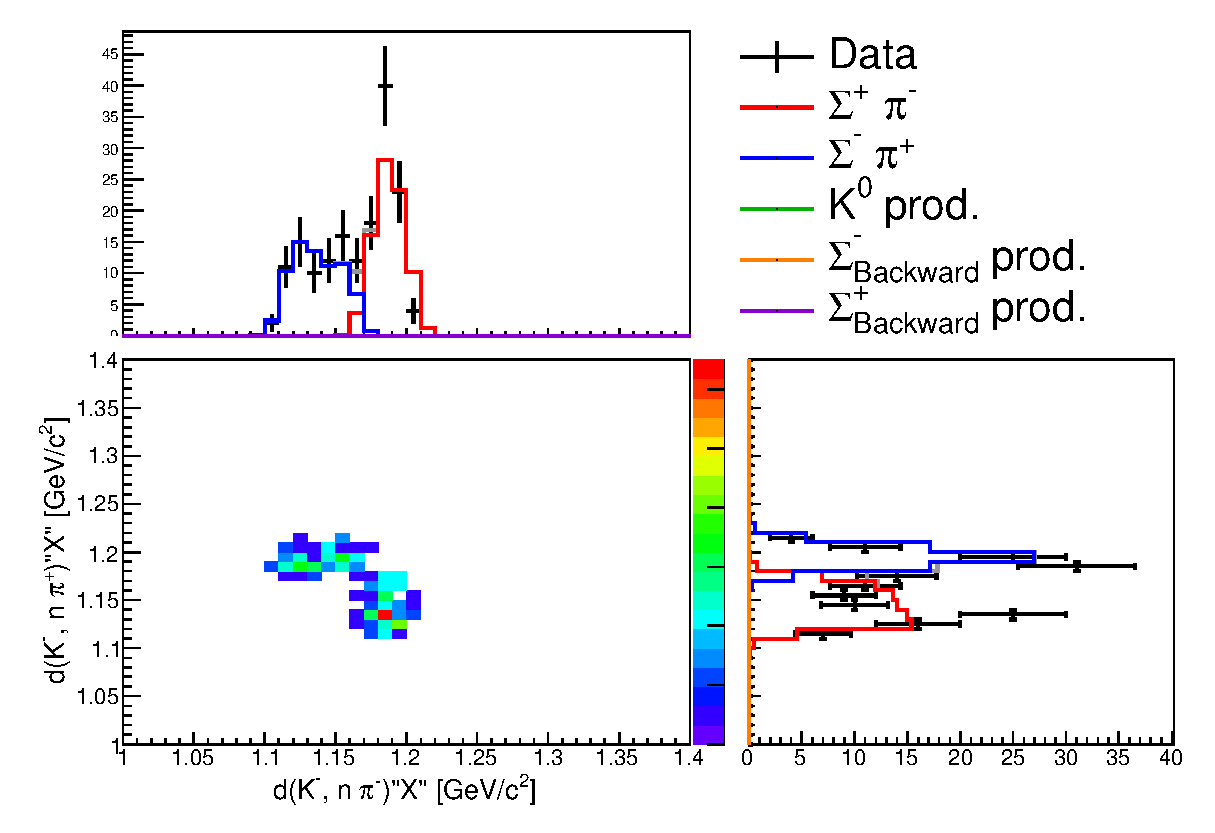
\includegraphics[width=4cm]{../pic/Run78/KN_ana_NC170_2sigma/KNpi_MM_4.eps}
    \end{minipage}
    \begin{minipage}{0.33\hsize}
      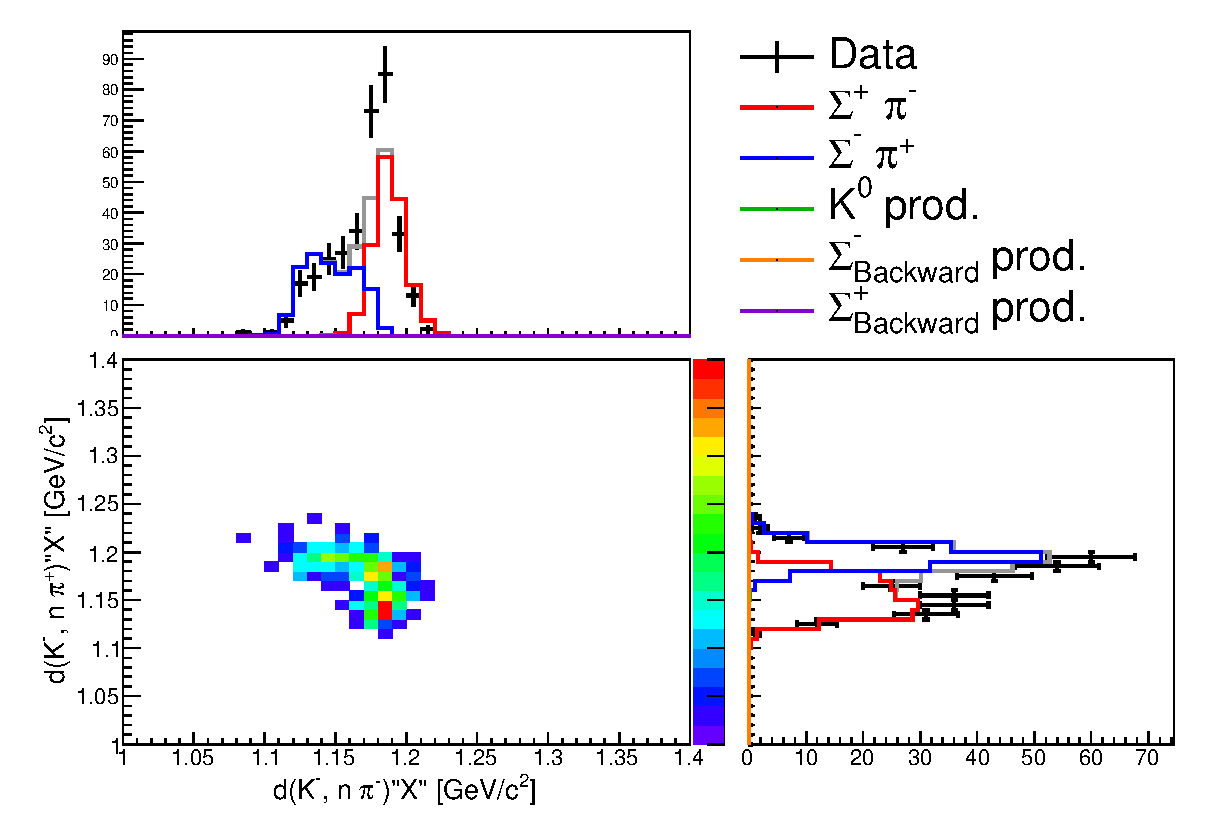
\includegraphics[width=4cm]{../pic/Run78/KN_ana_NC170_2sigma/KNpi_MM_5.eps}
    \end{minipage}    
  \end{tabular}

  \begin{tabular}{ccc}
    \begin{minipage}{0.33\hsize}
      \includegraphics[width=4cm]{../pic/Run78/KN_ana_NC170_2sigma/KNpi_MM_6.eps}
    \end{minipage}
    \begin{minipage}{0.33\hsize}
      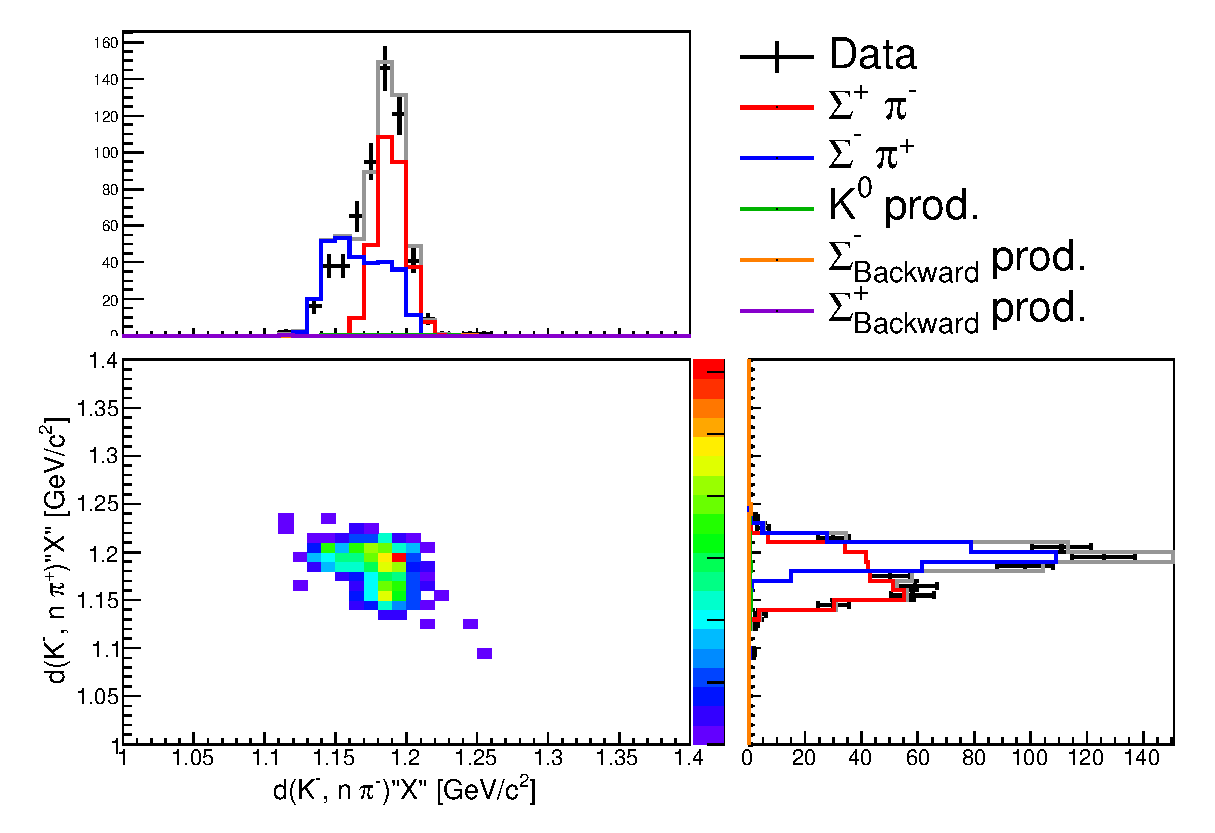
\includegraphics[width=4cm]{../pic/Run78/KN_ana_NC170_2sigma/KNpi_MM_7.eps}
    \end{minipage}
    \begin{minipage}{0.33\hsize}
      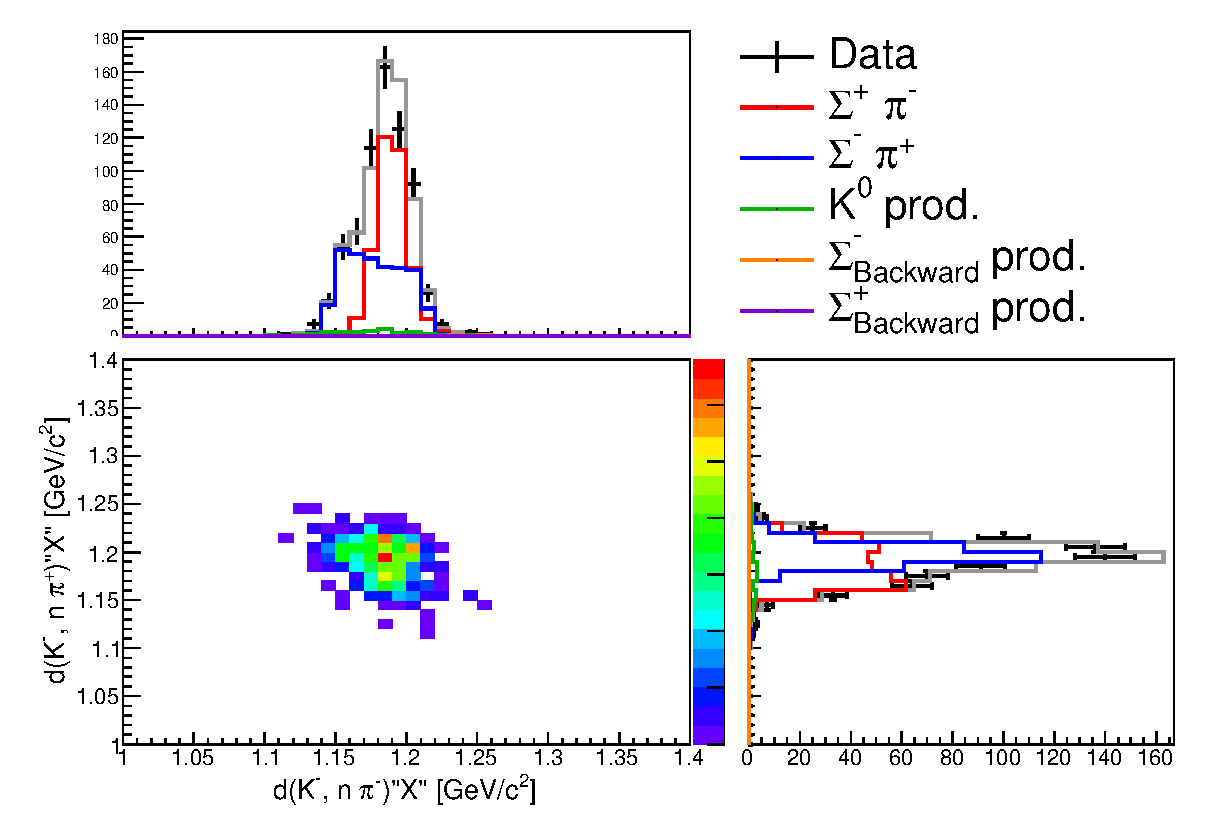
\includegraphics[width=4cm]{../pic/Run78/KN_ana_NC170_2sigma/KNpi_MM_8.eps}
    \end{minipage}    
  \end{tabular}

  \begin{tabular}{ccc}
    \begin{minipage}{0.33\hsize}
      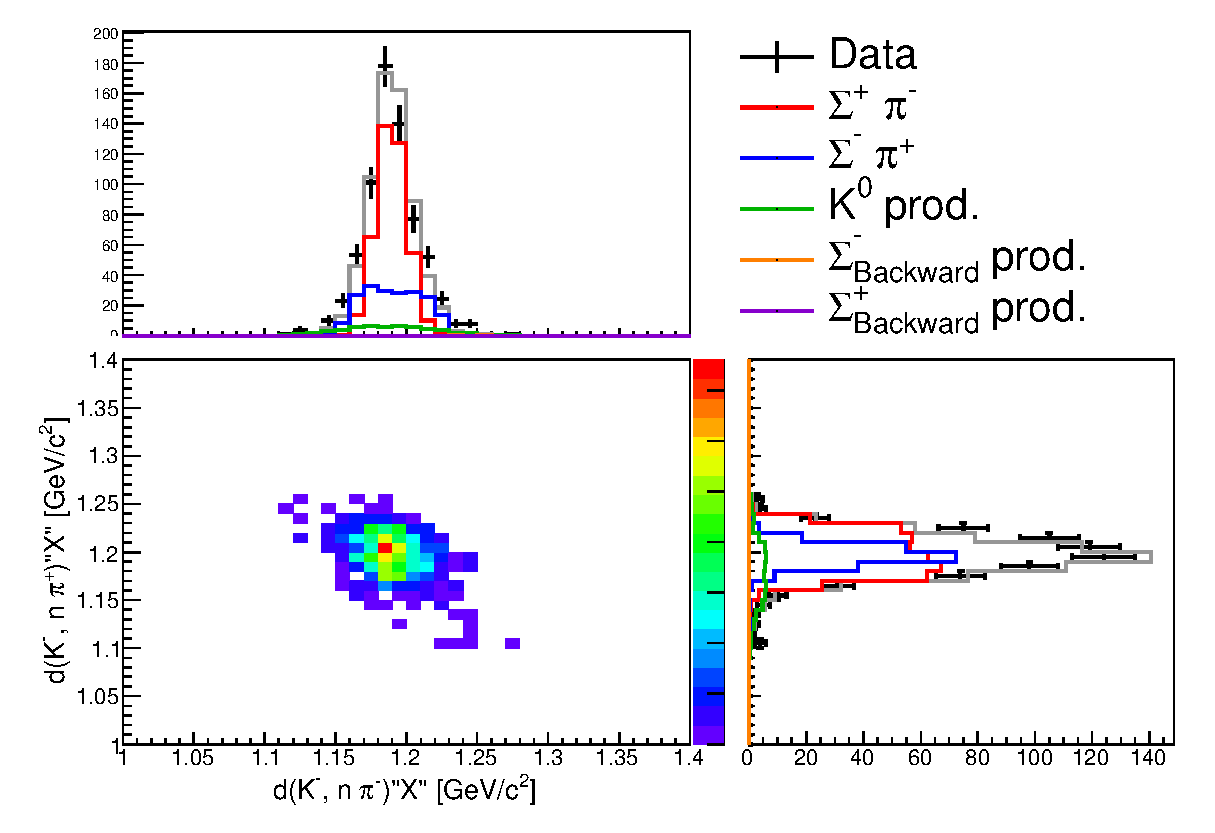
\includegraphics[width=4cm]{../pic/Run78/KN_ana_NC170_2sigma/KNpi_MM_9.eps}
    \end{minipage}
    \begin{minipage}{0.33\hsize}
      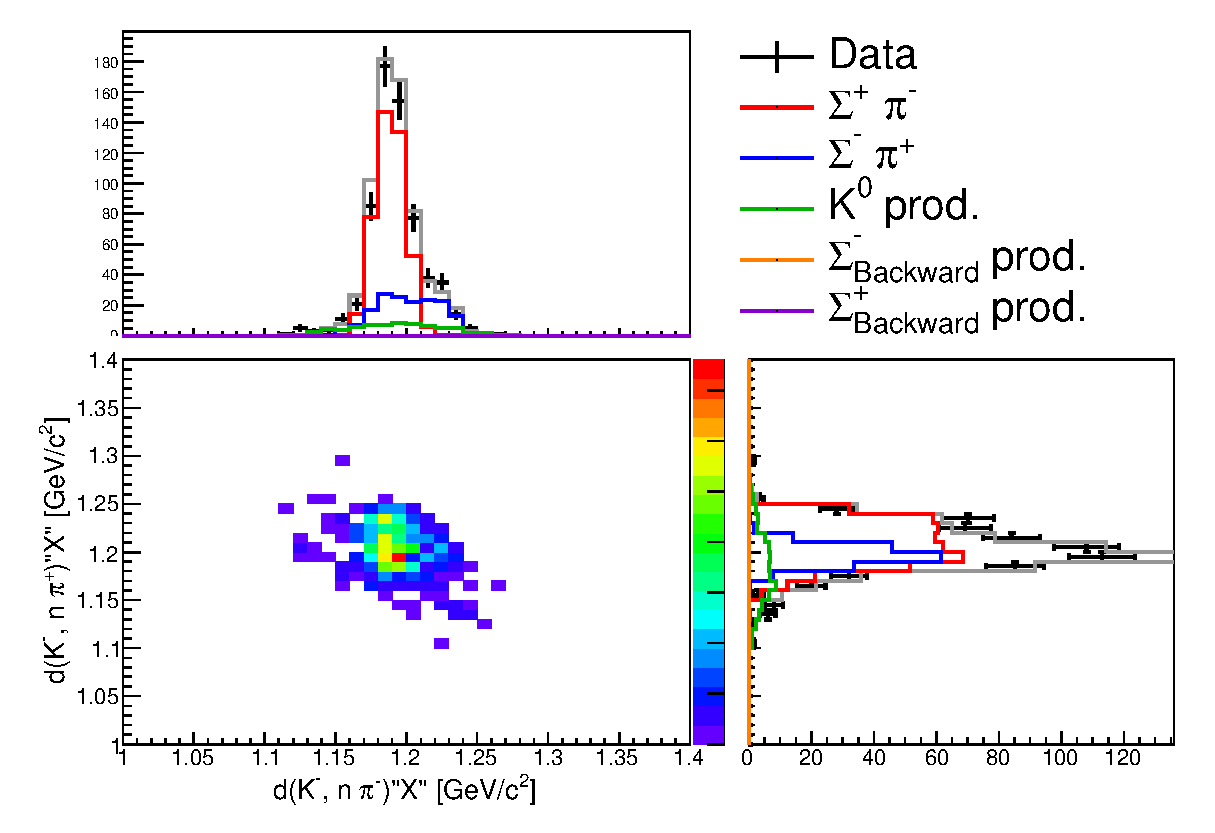
\includegraphics[width=4cm]{../pic/Run78/KN_ana_NC170_2sigma/KNpi_MM_10.eps}
    \end{minipage}
    \begin{minipage}{0.33\hsize}
      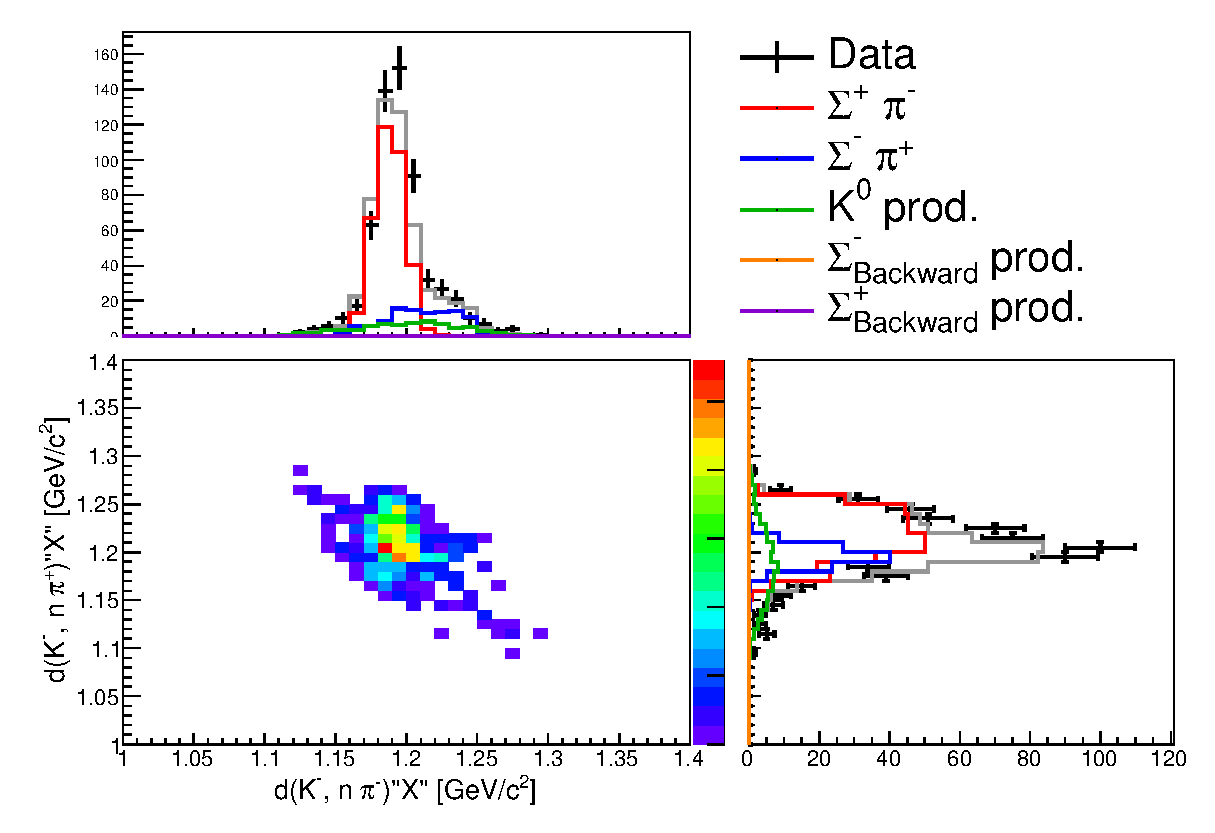
\includegraphics[width=4cm]{../pic/Run78/KN_ana_NC170_2sigma/KNpi_MM_11.eps}
    \end{minipage}    
  \end{tabular}

  \begin{tabular}{ccc}
    \begin{minipage}{0.33\hsize}
      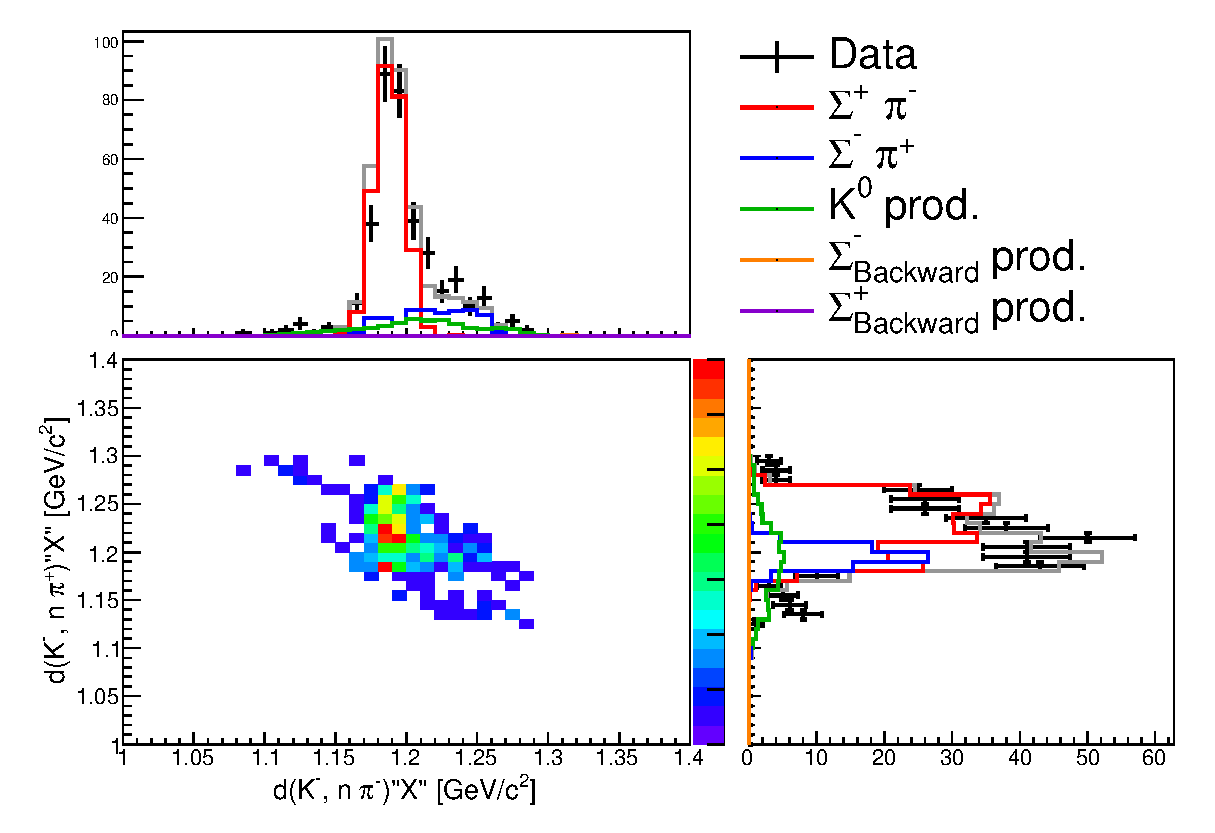
\includegraphics[width=4cm]{../pic/Run78/KN_ana_NC170_2sigma/KNpi_MM_12.eps}
    \end{minipage}
    \begin{minipage}{0.33\hsize}
      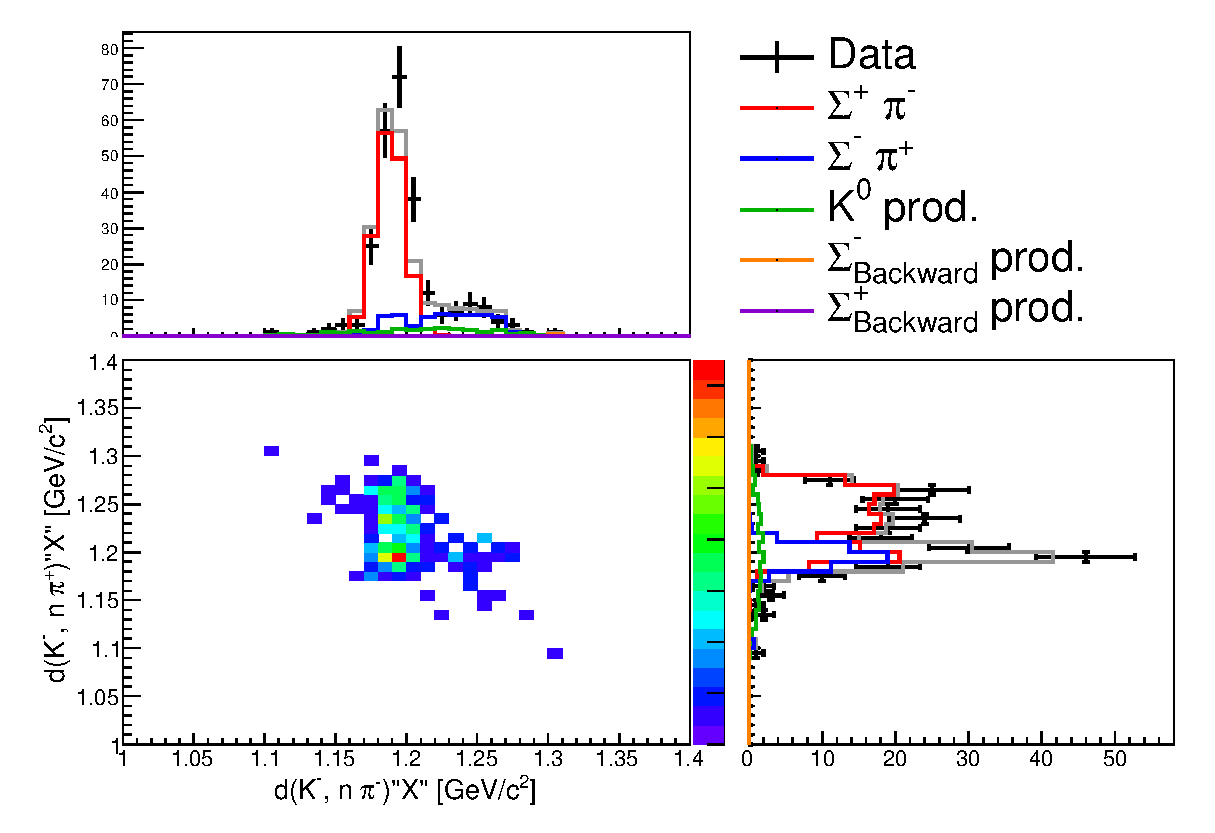
\includegraphics[width=4cm]{../pic/Run78/KN_ana_NC170_2sigma/KNpi_MM_13.eps}
    \end{minipage}
    \begin{minipage}{0.33\hsize}
      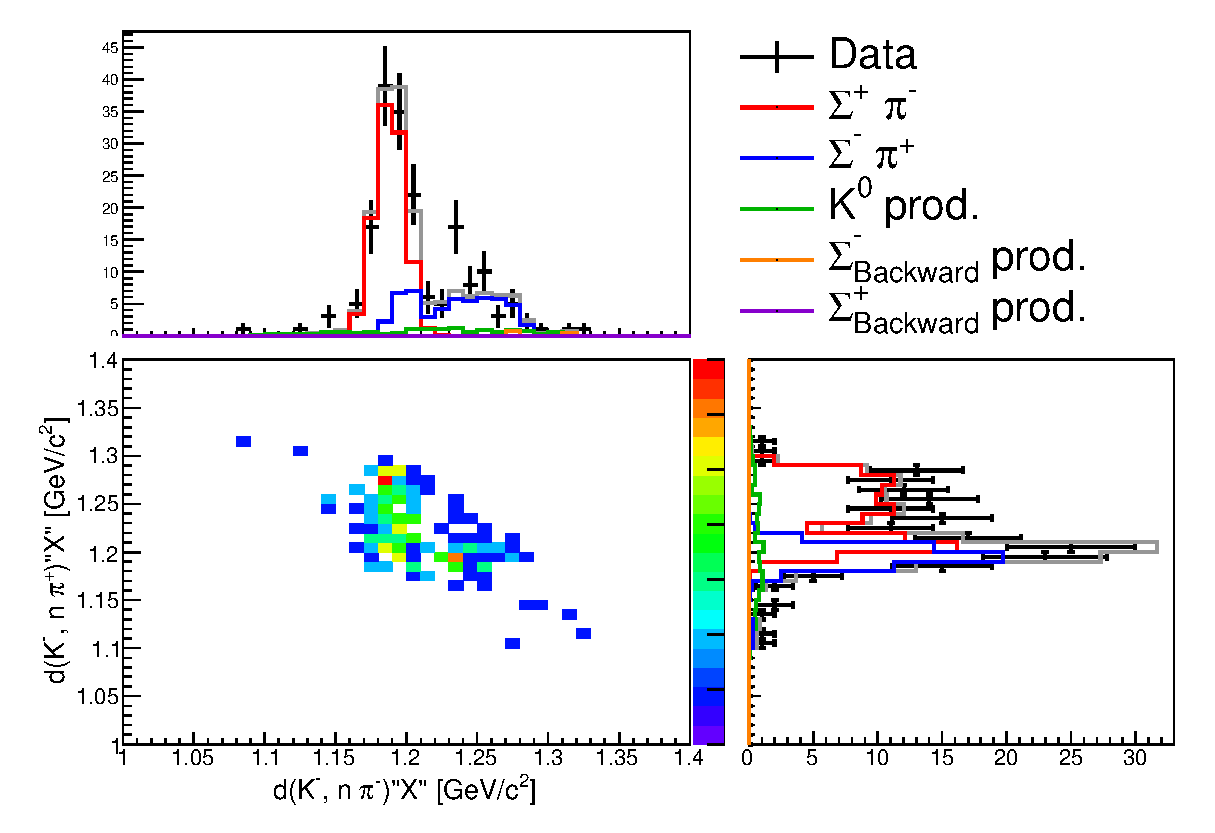
\includegraphics[width=4cm]{../pic/Run78/KN_ana_NC170_2sigma/KNpi_MM_14.eps}
    \end{minipage}    
  \end{tabular}

  \begin{tabular}{ccc}
    \begin{minipage}{0.33\hsize}
      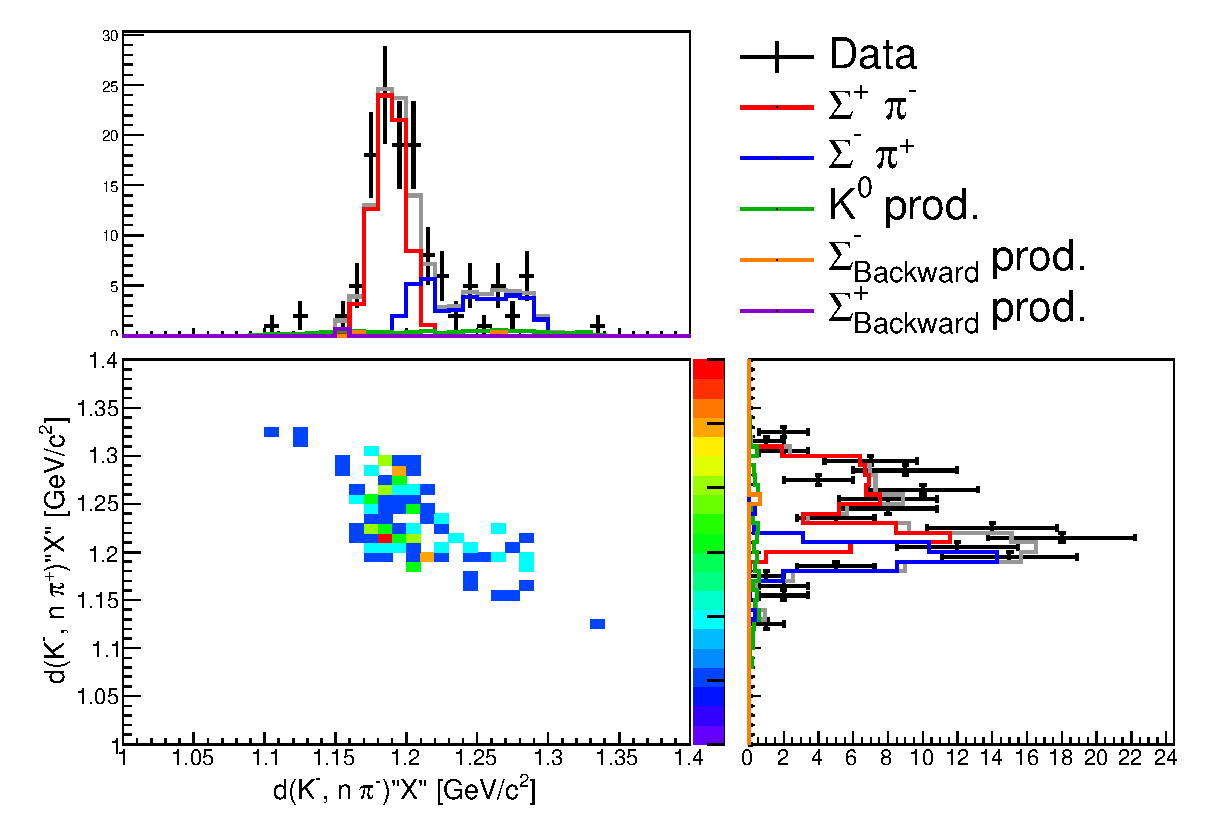
\includegraphics[width=4cm]{../pic/Run78/KN_ana_NC170_2sigma/KNpi_MM_15.eps}
    \end{minipage}
    \begin{minipage}{0.66\hsize}
      % Blank 
    \end{minipage}    
  \end{tabular}
  
  \caption{
    These figures indicate fitting results of each bins of $d(K^-, n)"\pi^{\mp}\Sigma^{\pm}"$ whose bin width is $10 MeV/c^2$.    
    Upper left figure shows about $1.35\sim1.36 GeV/c^2$ bin and the figure just to the right shows about $1.36\sim1.37 GeV/c^2$ bin.
    So, lower left figure shows about $1.49\sim1.50 GeV/c^2$ bin.
  }
  \label{fig:KNpi_MM_fit_div}
\end{figure}





Reacion.(\ref{eq:KD_K0nn})-(\ref{eq:KD_pipSm}) were decomposed by the so-called template fitting using the TFractionFitter of the ROOT \cite{tempfit},
and the error estimation was according to this reference \cite{pitfall_tempfit}.
For this decomposition, we simulated following reactions.
\begin{eqnarray}
  K^- d \rightarrow K^0 n n_{spectator} \label{eq:KD_K0nns}\\
  K^- d \rightarrow \Sigma^{+} \pi^- n_{spectator} \label{eq:KD_pimSp_ns} \\
  K^- d \rightarrow \Sigma^{-} \pi^+ n_{spectator} \label{eq:KD_pipSm_ns} \\
  K^- d \rightarrow n_{forward} (\Sigma^+ \pi^{-}) \label{eq:KD_nf_pimSp} \\
  K^- d \rightarrow n_{forward} (\Sigma^- \pi^{+}) \label{eq:KD_nf_pipSm} 
\end{eqnarray}
Reaction.(\ref{eq:KD_K0nns})-(\ref{eq:KD_pipSm_ns}) were 1-step reactions, so the neutron works as the spectator and according to momentum distribution of the fermi motion in the deuteron.
The fermi motion was simulated according to the previous experiment result which using the $d(e, e' p)"n"$ reaction\cite{d_fermi_ex}.
The angular distribution of the 1-nucleous $K^- N$ reaction have been studied about various final states and widly energy region\cite{CERN_HARA_K}.
Of course, the $K^- p \rightarrow K^0 n$ and the $K^- p \rightarrow \Sigma^{\pm} \pi^{\mp}$ with 1$GeV/c$ $K^-$ beam have been studied and
the angular distribution was published by this articles \cite{KP_MB}.
These angular distributions were used in our simulation.
On the other hand, The 2-step reaction of the $K^- d \rightarrow n \Sigma^{\pm} \pi^{\mp}$ has been not measured, so there are no data.
In this simulation, the neutron was emitted at a forward angle ($\theta<8^{\circ}$) which almost corresponded to the aperture of the Ushiwaka,
and the redidual $\pi\Sigma$ state was isotropically decayed.
These scattering strengths were depended on the $\pi\Sigma$ mass and there no data.
So, these data should be determined from our data.
So these data should be determined from our data, the decomposition of the $d(K^-, n \pi^+ \pi^-)"n"$ events was performed for this purpose.

The decomposition was performed	by 2 stages which of one is the identification of the 1-step reactions Reaction.(\ref{eq:KD_pimSp_ns})-(\ref{eq:KD_pipSm_ns})
and the other is the 2-step reaction decomposition of the $d(K^-, n)"\pi^-\Sigma^+"$ mode and the $d(K^-, n)"\pi^+\Sigma^-$ mode.
These fittings were performed internationally.
The identification of the 1-step reaction was performed to fit the invariant masses of $\pi^+$ $\pi^-$, $n$ $\pi^+$, and $n$ $\pi^-$.
In this fitting, the strength of the $d(K^-, n)"\pi^{\mp}\Sigma^{\pm}"$ was fixed
and the number of free parameters was tree which is each strength of the Reaction.(\ref{eq:KD_K0nns})-(\ref{eq:KD_pipSm_ns}),
which was performed as Fig\ref{fig:IM_fit}

\begin{figure}[htbp]
  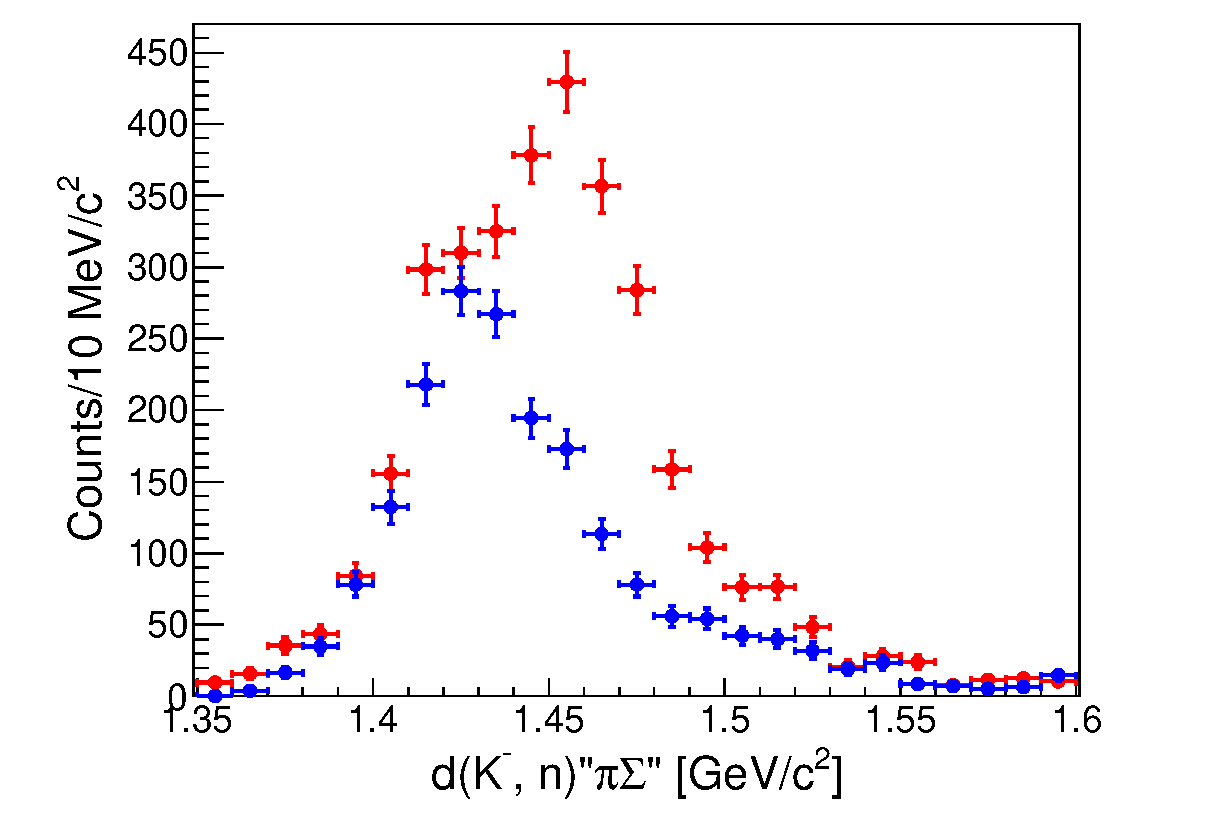
\includegraphics[width=12cm]{../pic/Run78/K0_ts_L1520/before_after.eps}
  \caption{
    This figure indicates decomposed number of $d(K^-, n)"\pi^-\Sigma^+"$ and $d(K^-, n)"\pi^+\Sigma^-"$ modes.
    In this figure, $K^0$ 2-step reaction effect is including which discribed Sec.\ref{sec:K0_2step}.
  }
  \label{fig:ChargeNum}
\end{figure}

The decomposition of the $d(K^-, n)"\pi^{\mp}\Sigma^{\pm}"$ modes was performed by the fittings of the $d(K^-, n \pi^{\mp})"\Sigma^{\pm}"$.
In this fitting, strengths of Reaction.(\ref{eq:KD_K0nns})-(\ref{eq:KD_pipSm_ns}) were fixed
and the number of free parameters was two which is the strengths of the $d(K^-, n)"\pi^{\mp}\Sigma^{\pm}"$ modes.
These missing masses give the missing $\Sigma$ peak if the correct charge combination.
For example, in the $d(K^-, n)"\pi^- \Sigma^+"$ mode,
the missing mass of the $d(K^-, n \pi^-)"n"$ gave the missing $\Sigma^+"$ peak,
and in the opposite charge, that made a broad distribution, which was shown as the left figure of Fig\ref{fig:KNpi_MM_fit}.
Because the relative strength of the $d(K^-, n)"\pi^{\mp}\Sigma^{\pm}"$ was depends on the $\pi \Sigma$ mass, this fitting was performed bin-by-bin of the $d(K^-, n)$ missing mass.
Fig\ref{fig:KNpi_MM_fit} represents the fitting result, in which the left figure shows summed up of all bins result and the right figure shows the log-likelihood value of each fitting.
Each fitting results were shown in Fig\ref{fig:KNpi_MM_fit_div}.
We obtained the decomposed spectra of the $d(K^-, n)"\pi^{\mp}\Sigma^{\pm}"$ as the result of the fitting, which represents in Fig\ref{fig:ChargeNum}.

The obtained counts convert to the differential cross section to estimated the acceptance of the CDS about the produced $\pi^{\mp} \Sigma^{\pm}$ states.
For the estimation, the simulation of Reaction.(\ref{eq:KD_nf_pimSp}-\ref{eq:KD_nf_pipSm}) were used.
Because the acceptance was about the CDS, events that can be analyzed about the forward scattered neutron were adopted as the trigger.
These events were adopted the same analysis procedure about the real data,
so the acceptance included analysis efficiencies about the particle identification of the CDS,
the $d(K^-, n \pi^+ \pi^-)"n"$ selection and rejection of the $K^0$ and the $\Sigma^{\pm}_{forward}$ and so on.
Fig \ref{fig:Acc_piS} shows the efficiency of $d(K^-, n)"\pi^{\mp}\Sigma^{\pm}"$ modes whose horizontal axis indicates generated $\pi \Sigma$ masses,
and Fig \ref{fig:piS_num} represents the acceptance corrected spectra.

\begin{figure}[htbp]
  \centering
  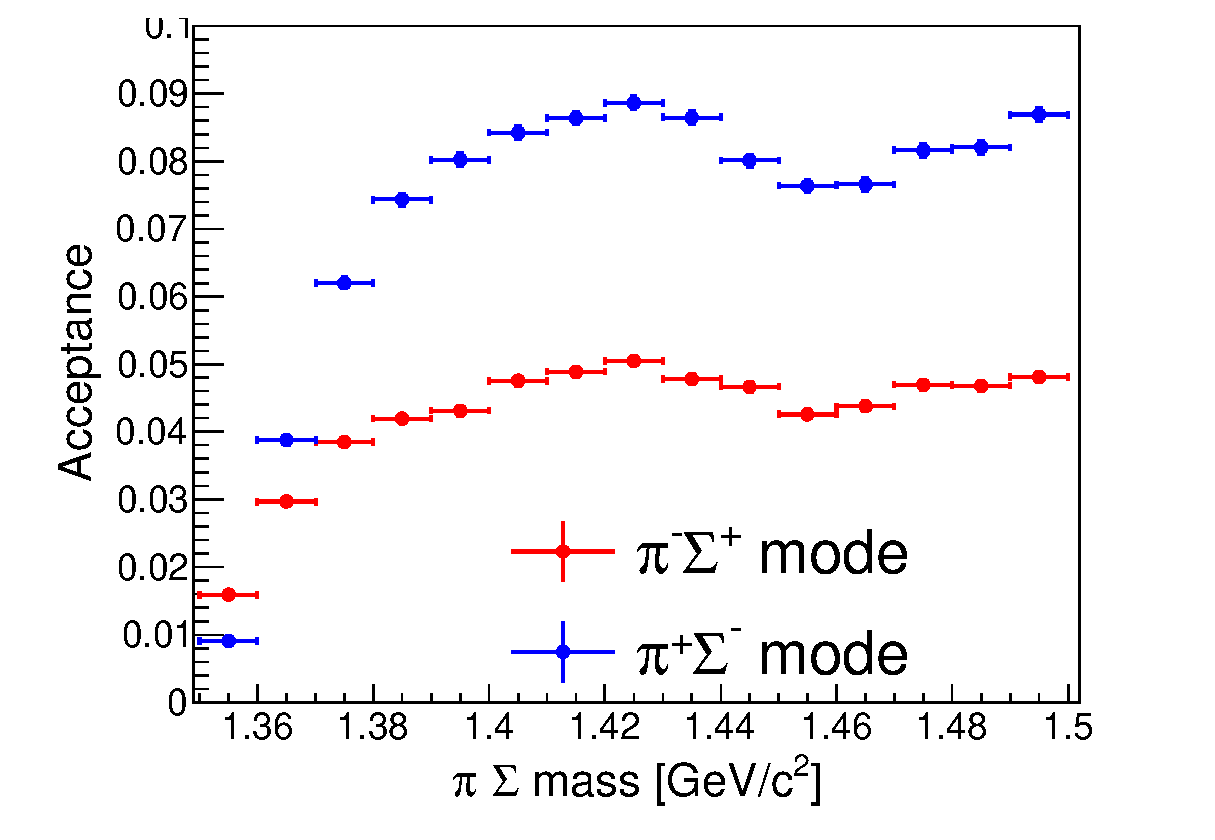
\includegraphics[width=8cm]{../pic/Run78/KN_ana_NC170_2sigma/kn_acc.eps}
  \caption{
    This figure represents the acceptance of the CDS estimated using the Monte Carlo simulation.
    The horizontal axis represents the generated $\pi^{\mp} \Sigma^{\pm}$ mass.
    The efficiency was judged by the same analysis procedure of the real data.
  }
  \label{fig:Acc_piS}
\end{figure}

\begin{figure}[htbp]
  \centering
  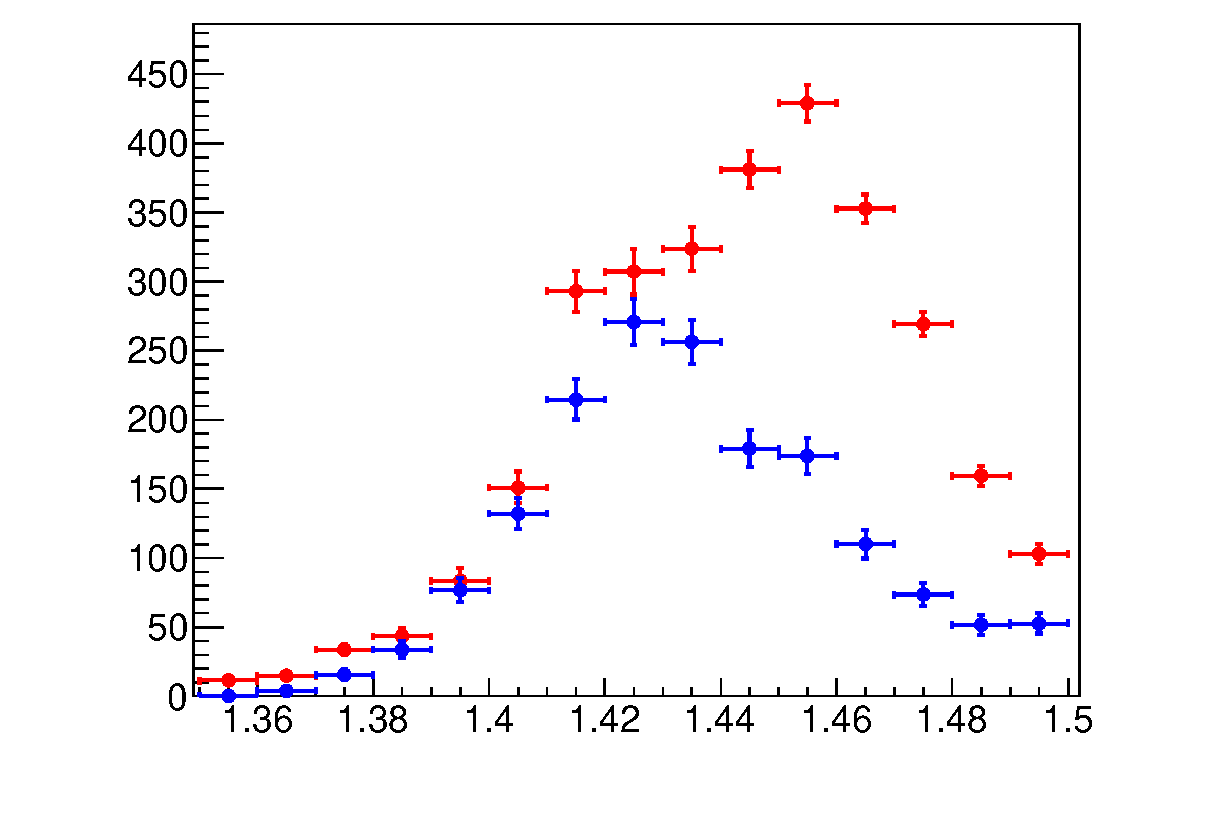
\includegraphics[width=8cm]{../pic/Run78/KN_ana_NC170_2sigma/piS_num.eps}
  \caption{
    This figue shows the acceptance corrected spectra.
  }
  \label{fig:piS_num}
\end{figure}
